\documentclass[%margin%,line,pifont,palatino,courier
]{article}
\usepackage{fullpage}
\usepackage{lastpage}
\usepackage[top=1in,bottom=1in,margin=1in]{geometry}
\usepackage{supertabular}
\usepackage{graphicx,tikz}	
%\usepackage{tkz-euclide}
%\usetkzobj{all}
%\usetikzlibrary{calc}
\usepackage{array,multicol}
\usepackage{amsmath,amssymb}
\usepackage{enumitem}
\usepackage{framed}

\usepackage{fancyhdr}
\pagestyle{fancy}

\addtolength{\topmargin}{-0.25in}

\newcommand{\vect}[1]{\mathbf{#1}}
\DeclareMathOperator{\proj}{proj}

\fancypagestyle{plain}{
	\addtolength{\headheight}{0.485in}
	\rhead{\bf MATH 2574 (Calculus III) \\
		%\vspace{0.5pc}
		due Mon 13 Mar 2017 \\}
	\rfoot{\footnotesize $\;$Quiz 6TH, p. \thepage\ (of \pageref{LastPage})
	}
\renewcommand{\headrulewidth}{0pt}
}
\fancyhf{}
\renewcommand{\headrulewidth}{0pt}
\rfoot{\footnotesize Quiz 6TH, p. \thepage\ (of \pageref{LastPage})$\;$}

\title{\vspace{-3.5pc} 
	\flushleft \bf \Large Take-Home Quiz 6: \\ Double and triple integrals (\S 13.2, 13.4-13.5)}
\date{}

% % % % %
\begin{document}
\maketitle

\vspace{-3pc}
\noindent{\bf Directions:} This quiz is due on March 13, 2017 at the beginning of lecture.  You may use whatever resources you like -- e.g., other textbooks, websites, collaboration with classmates -- to complete it \textbf{but YOU MUST DOCUMENT YOUR SOURCES}.  Acceptable documentation is enough information for me to find the source myself.  Rote copying another's work is unacceptable, regardless of whether you document it.  

\noindent\hrulefill

\begin{enumerate}
% % %
\item {\bf 13.2 \#70}
Find the volume of the solid above the parabolic region
\[
R=\{(x,y)\mid 0\leq x\leq 1,\, 0\leq y\leq 1-x^2\}
\]
and between the planes $z=1$ and $z=2-y$ (see figure).

\begin{center}
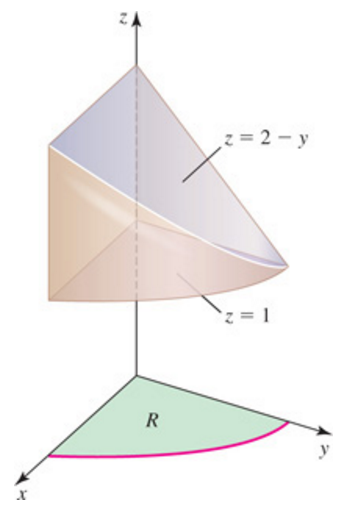
\includegraphics[scale=0.75]{Q613-2}
\end{center}

% % %
\item {\bf 13.4 \#50}
Use another order of integration to evaluate
\[
\int_1^4\int_z^{4z}\int_0^{\pi^2} \frac{\sin{\sqrt{yz}}}{x^{\frac{3}{2}}}\ dy\ dx\ dz.
\]

% % %
\item {\bf 13.5 \#16}
Use cylindrical coordinates to evaluate
\[
\int_0^3\int_{-\sqrt{9-y^2}}^{\sqrt{9-y^2}}\int_0^{9-3\sqrt{x^2+y^2}}\ dz\ dx\ dy.
\]

\newpage
% % %
\item {\bf 13.5 \#48}
Use spherical coordinates to find the volume of the solid cardiod of revolution (see figure)
\[
D=\{(\rho,\varphi,\theta)\mid 0\leq\rho\leq 1+\cos{\varphi},\, 0\leq\varphi\leq\pi,\, 0\leq \theta\leq 2\pi\}.
\]

\begin{center}
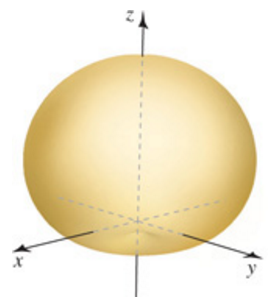
\includegraphics[scale=0.75]{Q6cardiod}
\end{center}

% % %
\item {\bf 13.5 \#76}
Before a gasline-powered engine is started, water must be drained from the bottom of the fuel tank (see figure).  Suppose the tank is a right circular cylinder on its side with a length of 2 ft and a radius of 1 ft.  If the water level is 6 in above the lowest part of the tank, determine how much water must be drained from the tank.

\begin{center}
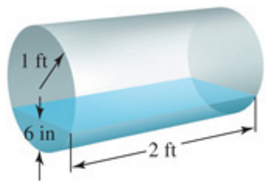
\includegraphics[scale=1]{Q6tank}
\end{center}

% % % % %
\end{enumerate}
\end{document}